\documentclass{jarticle}
\usepackage[dvipdfmx]{graphicx}
\usepackage[top=30truemm,bottom=30truemm,left=25truemm,right=25truemm]{geometry}
% \usepackage{here}
\usepackage{ascmac}

\title{14班企画書}
\author{細野虎太郎 小嶋樹 早道広峻 谷口隼輔}

\begin{document}

\maketitle

\section{概略}
このゲームは最初、プレイヤーが同じ場所から同時に一斉にスタートし、同じゴールを目指す。
ゴールまでの道のりは必ずしも平たんとは限らない。例えば谷が存在した場合には橋をかけたり、
丘が存在した場合、プロックを使って乗り越えるか、迂回するかを自分で決め、プレイヤーはその道を進んでゴールを目指す。
表~\ref{table:rule}にゲームの仕様とルールを示しておく!
\begin{table}[h]
    \caption{ゲームのおおまかな仕様とルール}
    \label{table:rule}
    \begin{center}
    \begin{tabular}{|l|l|}\hline
    ゲームジャンル & レースアクションゲーム\\
    プレイヤー人数 & 2 ~ 5 人              \\
    ゲームに対するルール & 自分以外の全潜水艦が撃沈した時点で終了する \\ \hline
    \end{tabular}
    \end{center}
\end{table}

\section{コンセプト}
\label{コンセプト}
このゲームのコンセプトは『自分の道は自分で決めろ!』である.
指先だけでなく体重移動まで使った特徴的な操作や,
自由なブロックの設置を通じて,プレイヤーの数だけ正しいルートがある全く新しいレースゲーム.


\section{操作方法}
ゲームの操作は以下の入力機器のいずれかを用いる。
\begin{itemize}
    \item キーボード
    \item wiiリモコン
    \item バランスボード\&wiiリモコン
\end{itemize}

操作の種類は以下の通りである。
\begin{table}[h]
    \caption{操作方法1}
    \label{table:control1}
    \begin{center}
    \begin{tabular}{|l|l|l|}\hline
    操作 & キーボード & wiiリモコン\\ \hline
    加速 & W & 2 \\ \hline
    左右旋回 & AD & \verb+<->+ \\ \hline
    ジャンプ & Space & 振る or 1 \\ \hline
    ブロックの設置 & Enter & A \\ \hline
    ゲーム終了 & Escape& + \\\hline

    \end{tabular}
    \end{center}
\end{table}

\begin{table}[h]
    \caption{操作方法2}
    \label{table:control2}
    \begin{center}
    \begin{tabular}{|l|l|l|}\hline
    操作 & バランスボード\&wiiリモコン\\ \hline
    加速 & 2 \\ \hline
    左右旋回 & 体重移動 \\ \hline
    ジャンプ & 屈伸 or 振る or 1 \\ \hline
    ブロックの設置 & A \\ \hline
    ゲーム終了 & + \\\hline
    \end{tabular}
    \end{center}
\end{table}

\section{世界観の設定}
\begin{shadebox}
\label{世界観の設定}
西暦30xx年.Hayamich社\,とTaniguch社\,によって共同開発された
「ホバリングボード(通称 セグウェイ)」と「ブロック生成デバイス」を用いた
新たな娯楽がひそかに人気を集め始めていた.
(背景:
食料革命によって引き起こされた人口爆発は世界を手狭にさせた.
住む場所が足りなくなった人類は空中に地面を生成することに成功し,無限ともいえる居住区を手に入れた.
Taniguch社\,はこの技術を一般市民でも購入できる安価な機器として再開発した.さらに, Hayamich社\,はセグウェイを開発し空中の居住区間移動を従来からは考えられないほど劇的に容易なものとした.
スポーツマンをはじめとした人々はこのボード(セグウェイ)とデバイスを用いて観客を楽しませている.)
\end{shadebox}


\section{ゲームデータの構造}
以下にゲームデータの構造を示す
\begin{table}[h]
    \caption{クライアントのデータ構造}
    \label{table:data1}
    \begin{center}
    \begin{tabular}{|l||l|l|}\hline
    データ型 & 変数名 & 内容 \\ \hline
    char & \verb+name[MAX_LEN_NAME]+ & クライアントの名前 \\ \hline
    FloatCube & pos & マップ上の場所 \\ \hline
    int & rank & 順位 \\ \hline
    bool & goal & ゴールしているか \\ \hline
    \end{tabular}
    \end{center}
\end{table}
\begin{table}[h]
    \caption{ネットワークモジュール用のクライアントの情報}
    \label{table:data2}
    \begin{center}
    \begin{tabular}{|l||l|l|}\hline
    データ型 & 変数名 & 内容 \\ \hline
    int & connect & クライアントがサーバーに接続しているか \\ \hline
    int & sock & 使用するソケット \\ \hline
    struct sockaddr\_in & addr & ソケットの設定 \\ \hline
    \end{tabular}
    \end{center}
\end{table}
\begin{table}[h]
    \caption{クライアントの座標}
    \label{table:data3}
    \begin{center}
    \begin{tabular}{|l||l|l|}\hline
    データ型 & 変数名 & 内容 \\ \hline
    float & x & x座標 \\ \hline
    float & y & y座標 \\ \hline
    float & z & z座標 \\ \hline
    \end{tabular}
    \end{center}
\end{table}
\begin{table}[h]
    \caption{直方体形を定義する構造体}
    \label{table:data4}
    \begin{center}
    \begin{tabular}{|l||l|l|}\hline
    データ型 & 変数名 & 内容 \\ \hline
    float & x & x座標 \\ \hline
    float & y & y座標 \\ \hline
    float & z & z座標 \\ \hline
    float & w & x方向の長さ \\ \hline
    float & h & y方向の長さ \\ \hline
    float & d & z方向の長さ \\ \hline
    \end{tabular}
    \end{center}
\end{table}
\begin{table}[h]
    \caption{マップ用のデータ}
    \label{table:data5}
    \centering
    \begin{tabular}{|l||l|l|}\hline
    データ型 & 変数名 & 内容 \\ \hline
    int & \verb+_TerrainData+  & マップデータ \\
    & \verb+[MAP_SIZE_W][MAP_SIZE_H][MAP_SIZE_D]+ & \\ \hline
    \verb+vector<PlaceData>+ & \_ObjectDatas & オブジェクトデータ \\ \hline
    int & \_MapW & マップの横幅 \\ \hline
    int & \_MapH & マップの横縦 \\ \hline
    int & \_MapD & マップのサイズ \\ \hline
    \end{tabular}
\end{table}

\section{モジュール}
\subsection{サーバー}

以下に各モジュールの外部関数を説明する
\begin{enumerate}
    \item ネットワークモジュール
    \begin{table}[h]
        \label{table:fanc_s1-1}
        \begin{center}
            \begin{tabular}{|c||p{30em}|}\hline
                関数名&void SetupServer(int numCl, u\_short port)\\\hline
                機能&サーバーの初期設定を行う\\
                引数&numCl ―― クライアント数\\
                &port ―― ポート番号\\
                返り値&無し\\\hline
            \end{tabular}
        \end{center}
    \end{table}
    \begin{table}[h]
        \label{table:fanc_s1-2}
        \begin{center}
            \begin{tabular}{|c||p{30em}|}\hline
                関数名&int ControlRequests(void) \\\hline
                機能&クライアントからのリクエストに対応する\\
                引数&無し\\
                返り値&1:通信継続/0:通信終了\\\hline
            \end{tabular}
        \end{center}
    \end{table}
    \begin{table}[h]
        \label{table:fanc_s1-3}
        \begin{center}
            \begin{tabular}{|c||p{30em}|}\hline
                関数名&void RunCommand(int id, char com) \\\hline
                機能&コマンドの実行\\
                引数&id ―― 送信先のクライアントID\\
                &com ―― 送信するコマンド\\
                返り値&無し\\\hline
            \end{tabular}
        \end{center}
    \end{table}
    \begin{table}[h]
        \label{table:fanc_s1-4}
        \begin{center}
            \begin{tabular}{|c||p{30em}|}\hline
                関数名&void TerminateServer(void)  \\\hline
                機能&サーバーの終了処理を行う\\
                引数&無し\\
                返り値&無し\\\hline
            \end{tabular}
        \end{center}
    \end{table}
    \item マップモジュール
    \begin{table}[h]
        \label{table:fanc_s2-1}
        \begin{center}
            \begin{tabular}{|c||p{30em}|}\hline
                関数名&void LoadMapData(char* fileName)\\\hline
                機能&マップデータの読み込みを行う\\
                引数&fileName ―― マップデータファイル名\\
                返り値&無し\\\hline
            \end{tabular}
        \end{center}
    \end{table}
\end{enumerate}

\subsection{クライアント}

以下に各モジュールの外部関数を説明する
\begin{enumerate}
    \item ネットワークモジュール
    \begin{table}[h]
        \label{table:fanc_c1-1}
        \begin{center}
            \begin{tabular}{|c||p{30em}|}\hline
                関数名&void SetupClient(char *serverName, u\_short port) \\\hline
                機能&クライアントの初期設定を行う\\
                引数&serverName―― サーバー名\\
                &port ―― ポート番号\\
                返り値&無し\\\hline
            \end{tabular}
        \end{center}
    \end{table}
    \begin{table}[h]
        \label{table:fanc_c1-2}
        \begin{center}
            \begin{tabular}{|c||p{30em}|}\hline
                関数名&int ControlRequests(void) \\\hline
                機能&クライアントの制御を行う\\
                引数&無し\\
                返り値&1:通信継続/0:通信終了\\\hline
            \end{tabular}
        \end{center}
    \end{table}
    \begin{table}[h]
        \label{table:fanc_c1-3}
        \begin{center}
            \begin{tabular}{|c||p{30em}|}\hline
                関数名&int InCommand(char com) \\\hline
                機能&コマンドに対する処理を行う\\
                引数&com ―― コマンド\\
                返り値&1:通信継続/0:通信終了\\\hline
            \end{tabular}
        \end{center}
    \end{table}
    \begin{table}[h]
        \label{table:fanc_c1-4}
        \begin{center}
            \begin{tabular}{|c||p{30em}|}\hline
                関数名&void TerminateClient(void)  \\\hline
                機能&クライアントの終了処理を行う\\
                引数&無し\\
                返り値&無し\\\hline
            \end{tabular}
        \end{center}
    \end{table}

    \item システムモジュール
    \begin{table}[h]
        \label{table:fanc_s2-1}
        \begin{center}
            \begin{tabular}{|c||p{30em}|}\hline
                関数名&const PlayerData* GetPlayerData()\\\hline
                機能&プレイヤーデータ配列の先頭ポインタを返す\\
                引数&無し\\
                返り値&プレイヤーデータ配列の先頭ポインタ\\\hline
            \end{tabular}
        \end{center}
    \end{table}

    \item マップモジュール
    \begin{table}[h]
        \label{table:fanc_s3-1}
        \begin{center}
            \begin{tabular}{|c||p{30em}|}\hline
                関数名&SetMapData(int mapW,int mapH, int mapD, \\
                &int terrainData[MAP\_SIZE\_W][MAP\_SIZE\_H][MAP\_SIZE\_D])\\\hline
                機能&マップデータの初期設定を行う\\
                引数&mapW ―― マップの幅\\
                &mapH ―― マップの高さ\\
                &mapD ―― マップの奥行\\
                &terrainData ―― マップの地形データ\\
                返り値&無し\\\hline
            \end{tabular}
        \end{center}
    \end{table}

    \item 入力モジュール
    \begin{table}[h]
        \label{table:fanc_c4-1}
        \begin{center}
            \begin{tabular}{|c||p{30em}|}\hline
                関数名&virtual void GetInput(SDL\_Event event)\\\hline
                機能&ユーザー入力を受け取る\\
                引数&event ―― SDLのイベント\\
                返り値&無し\\\hline
            \end{tabular}
        \end{center}
    \end{table}
    \begin{table}[h]
        \label{table:fanc_c4-2}
        \begin{center}
            \begin{tabular}{|c||p{30em}|}\hline
                関数名&InputType GetInputType()\\\hline
                機能&現在の入力情報を返す\\
                引数&無し\\
                返り値&\_Input: 現在の入力情報\\\hline
            \end{tabular}
        \end{center}
    \end{table}
    \item グラフィックモジュール
    \begin{table}[h]
        \label{table:fanc_c5-1}
        \begin{center}
            \begin{tabular}{|c||p{30em}|}\hline
                関数名&void InitGraphic()\\\hline
                機能&グラフィックモジュールの初期設定を行う\\
                引数&無し\\
                返り値&無し\\\hline
            \end{tabular}
        \end{center}
    \end{table}
    \begin{table}[h]
        \label{table:fanc_c5-1}
        \begin{center}
            \begin{tabular}{|c||p{30em}|}\hline
                関数名&void Disp()\\\hline
                機能&グラフィックの表示を行う\\
                引数&無し\\
                返り値&無し\\\hline
            \end{tabular}
        \end{center}
    \end{table}

\end{enumerate}

\section{コマンドプロトコル}

\begin{enumerate}
    \item サーバー→クライアントのプロトコル
    \begin{table}[h]
        \label{table:command1-1}
        \begin{center}
            \begin{tabular}{|c||p{30em}|}\hline
                コマンド&M(PlayerData[])\\\hline
                機能&移動処理\\
                引数&全プレイヤーデータ\\
                対象&全クライアント\\
                タイミング&毎フレーム\\\hline
            \end{tabular}
        \end{center}
    \end{table}
    \begin{table}[h]
        \label{table:command1-2}
        \begin{center}
            \begin{tabular}{|c||p{30em}|}\hline
                コマンド&P(PlaceData)\\\hline
                機能&ブロックの設置\\
                引数&設置されたブロックのデータ\\
                対象&全クライアント\\
                タイミング&設置時\\\hline
            \end{tabular}
        \end{center}
    \end{table}
    \begin{table}[h]
        \label{table:command1-3}
        \begin{center}
            \begin{tabular}{|c||p{30em}|}\hline
                コマンド&D\\\hline
                機能&設置不可能\\
                引数&無し\\
                対象&クライアント\\
                タイミング&設置時\\\hline
            \end{tabular}
        \end{center}
    \end{table}
    \begin{table}[h]
        \label{table:command1-2}
        \begin{center}
            \begin{tabular}{|c||p{30em}|}\hline
                コマンド&G\\\hline
                機能&ゴールしたことを通知\\
                引数&なし\\
                対象&クライアント\\
                タイミング&ゴール時\\\hline
            \end{tabular}
        \end{center}
    \end{table}
    \begin{table}[h]
        \label{table:command1-2}
        \begin{center}
            \begin{tabular}{|c||p{30em}|}\hline
                コマンド&E(char[])\\\hline
                機能&エラーを通知\\
                引数&エラー内容\\
                対象&クライアント\\
                タイミング&エラー発生時\\\hline
            \end{tabular}
        \end{center}
    \end{table}
    \begin{table}[h]
        \label{table:command1-2}
        \begin{center}
            \begin{tabular}{|c||p{30em}|}\hline
                コマンド&F(PlayerData[])\\\hline
                機能&ゲームの終了を通知\\
                引数&全プレイヤーのデータ\\
                対象&全クライアント\\
                タイミング&全プレイヤーゴール時\\\hline
            \end{tabular}
        \end{center}
    \end{table}
    \begin{table}[h]
        \label{table:command1-3}
        \begin{center}
            \begin{tabular}{|c||p{30em}|}\hline
                コマンド&Q\\\hline
                機能&プログラムの強制終了\\
                引数&無し\\
                対象&全クライアント\\
                タイミング&任意\\\hline
            \end{tabular}
        \end{center}
    \end{table}

    \item クライアント→サーバーのプロトコル
    \begin{table}[h]
        \label{table:command2-1}
        \begin{center}
            \begin{tabular}{|c||p{30em}|}\hline
                コマンド&M(FloatPosition)\\\hline
                機能&移動処理\\
                引数&自身の移動後の座標\\
                対象&サーバー\\
                タイミング&毎フレーム\\\hline
            \end{tabular}
        \end{center}
    \end{table}
    \begin{table}[h]
        \label{table:command2-2}
        \begin{center}
            \begin{tabular}{|c||p{30em}|}\hline
                コマンド&P(PlaceData)\\\hline
                機能&ブロックの設置\\
                引数&設置するブロックのデータ\\
                対象&サーバー\\
                タイミング&設置時\\\hline
            \end{tabular}
        \end{center}
    \end{table}
    \begin{table}[h]
        \label{table:command2-3}
        \begin{center}
            \begin{tabular}{|c||p{30em}|}\hline
                コマンド&Q\\\hline
                機能&プログラムの強制終了\\
                引数&無し\\
                対象&サーバー\\
                タイミング&任意\\\hline
            \end{tabular}
        \end{center}
    \end{table}
\end{enumerate}

\section{スケジュール}

\section{ガントチャート}
\begin{figure}[h]
    \centering
    \label{table:gunt1}
    \caption{ガントチャート1}
    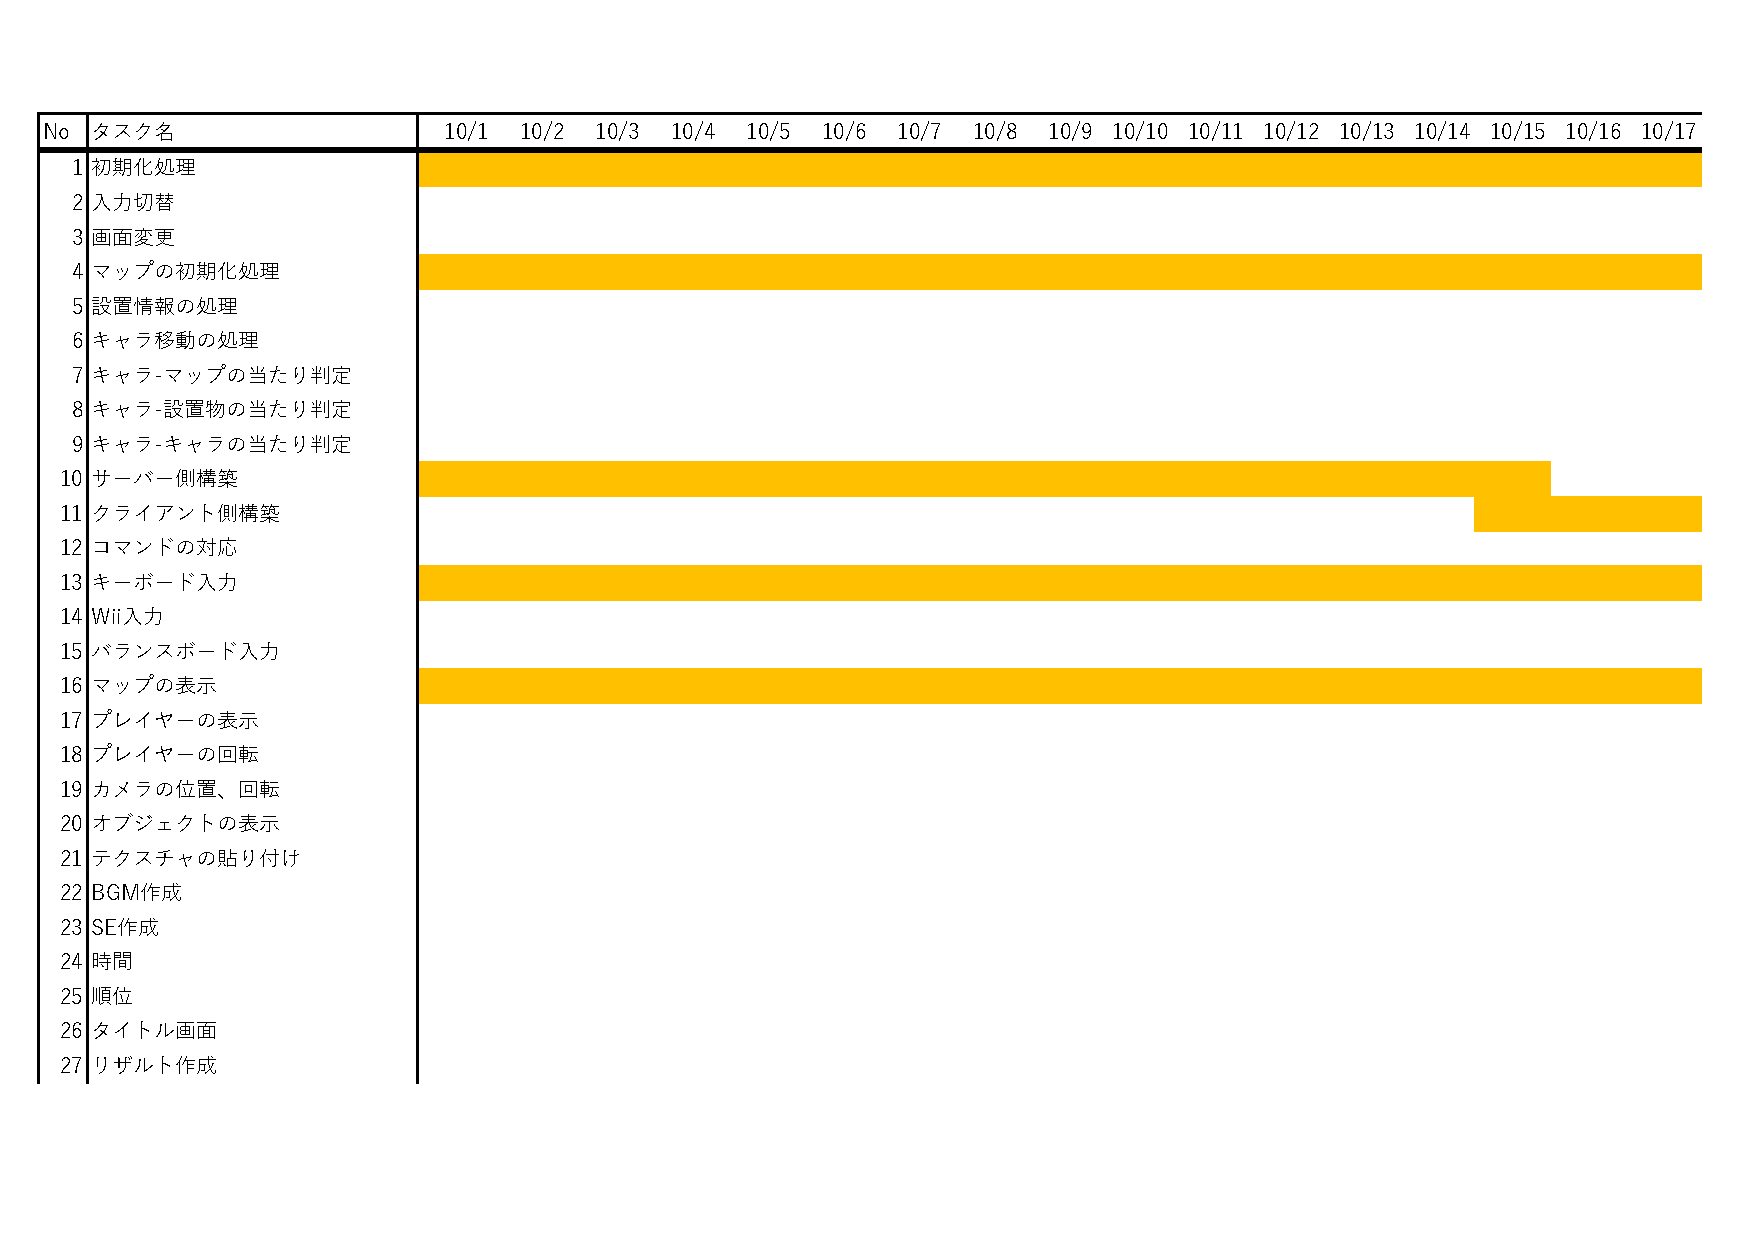
\includegraphics[scale=0.5, page=1]{gunt.pdf}
\end{figure}
\begin{figure}[h]
    \centering
    \label{table:gunt1}
    \caption{ガントチャート2}
    \includegraphics[scale=0.5, page=2]{gunt.pdf}
\end{figure}
\begin{figure}[h]
    \centering
    \label{table:gunt1}
    \caption{ガントチャート3}
    \includegraphics[scale=0.5, page=3]{gunt.pdf}
\end{figure}
\begin{figure}[h]
    \centering
    \label{table:gunt1}
    \caption{ガントチャート4}
    \includegraphics[scale=0.5, page=4]{gunt.pdf}
\end{figure}
\begin{figure}[h]
    \centering
    \label{table:gunt1}
    \caption{ガントチャート5}
    \includegraphics[scale=0.5, page=5]{gunt.pdf}
\end{figure}

\begin{figure}[h]
    \centering
    \label{table:gunt1}
    \caption{ガントチャートデータシート}
    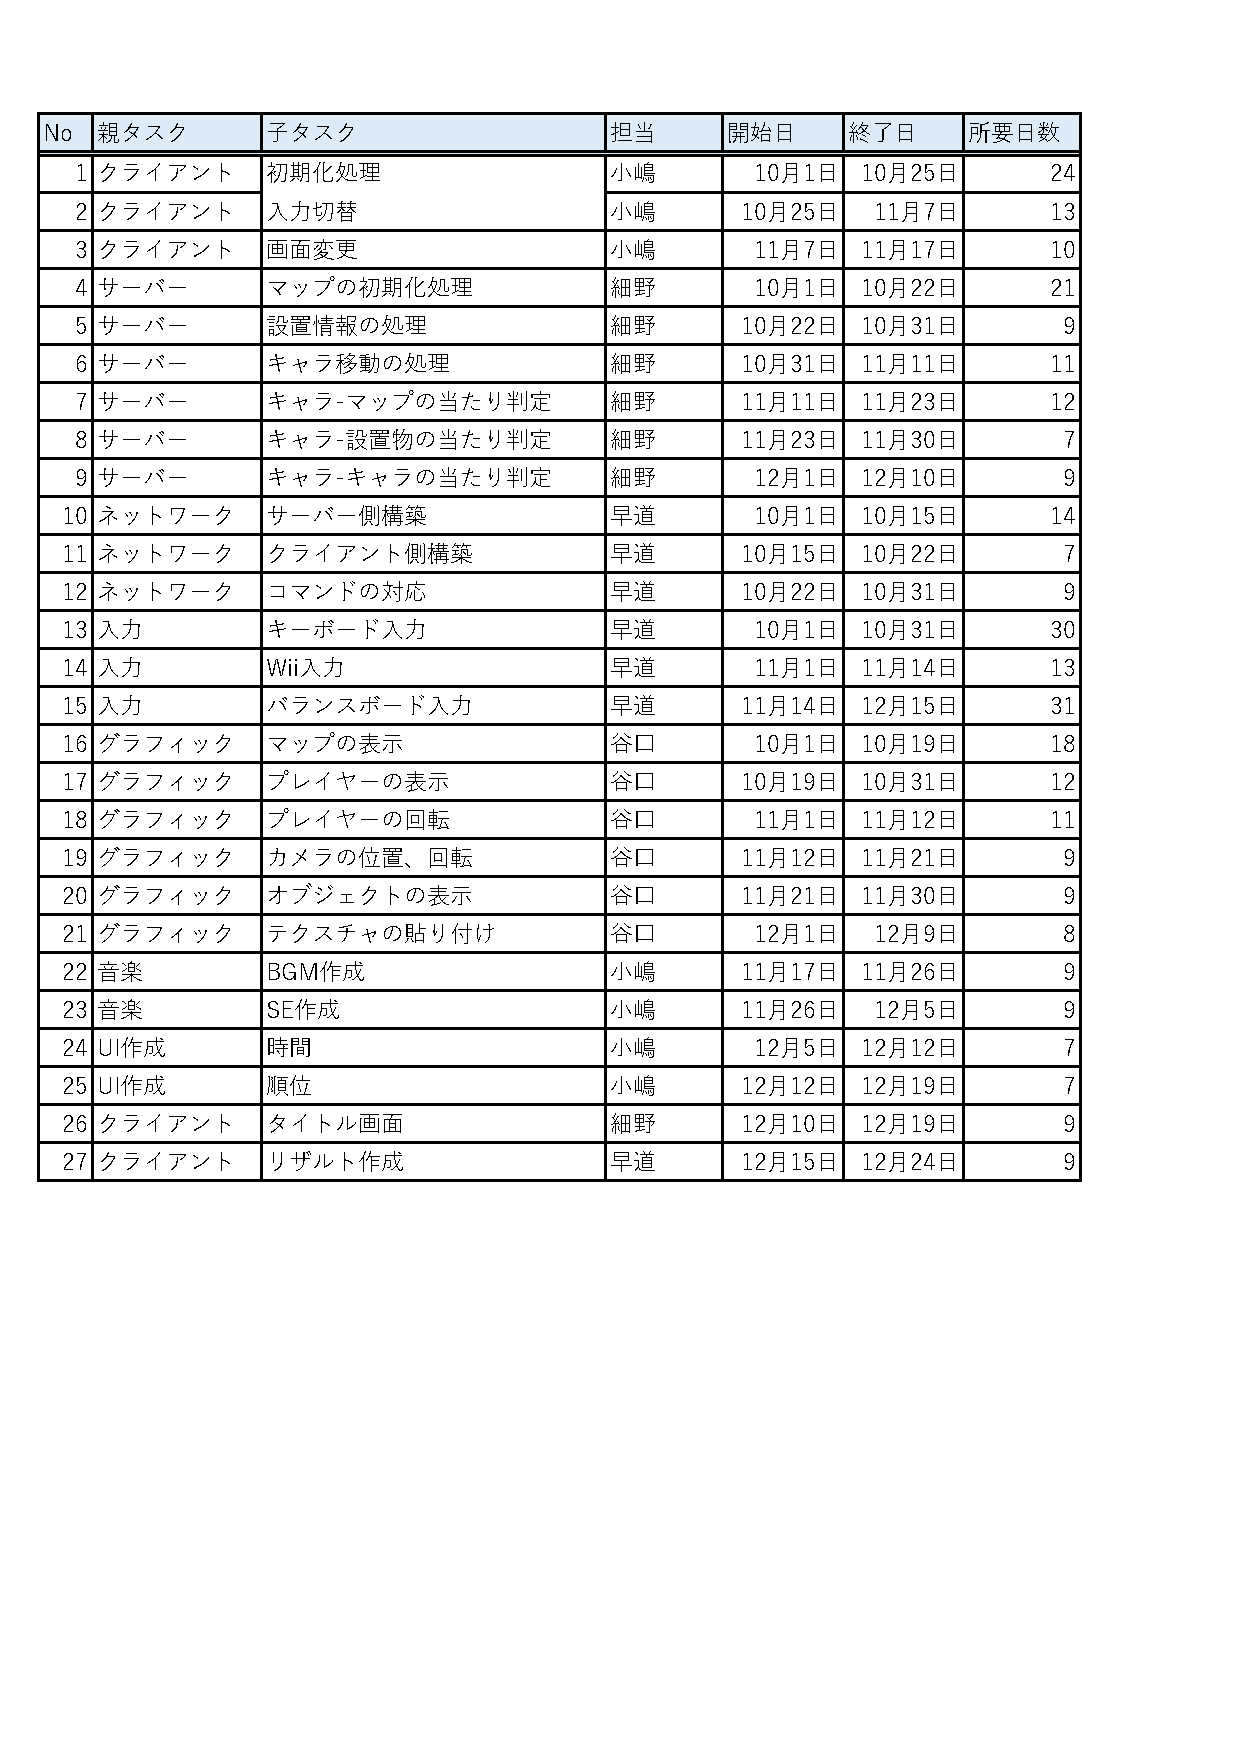
\includegraphics[scale=0.5]{guntdat.pdf}
\end{figure}


\end{document}
